\documentclass{beamer}

\usepackage[utf8]{inputenc}
\usepackage{hyperref}

\usetheme{Berkeley}
\beamertemplatenavigationsymbolsempty
\setbeamertemplate{headline}{}
 
\title{Erstellen eines Workflows in FoodChain-Lab 1}
\date{}
 
\begin{document}
\maketitle

\section{ }

\subsection{Aufgaben}
\begin{frame}
	\begin{itemize}
		\item Importieren Sie das Beispiel-Excel-Template von: \url{https://github.com/SiLeBAT/BfROpenLabResources/raw/master/GitHubPages/documents/fake_data.xls}
		\item Vergeben mit Hilfe des \textbf{Tracing}-Knotens ein Gewicht ("Weight") von "1" an die Supermärkte in Hamburg, Ingolstadt und Münster um diese als Ausbruchsorte zu markieren.
		\item Nutzen Sie den \textbf{Tracing View} um das Liefernetz zu visualisieren.
	\end{itemize}
\end{frame}
 
\subsection{1}
\begin{frame}
	\begin{center}
  		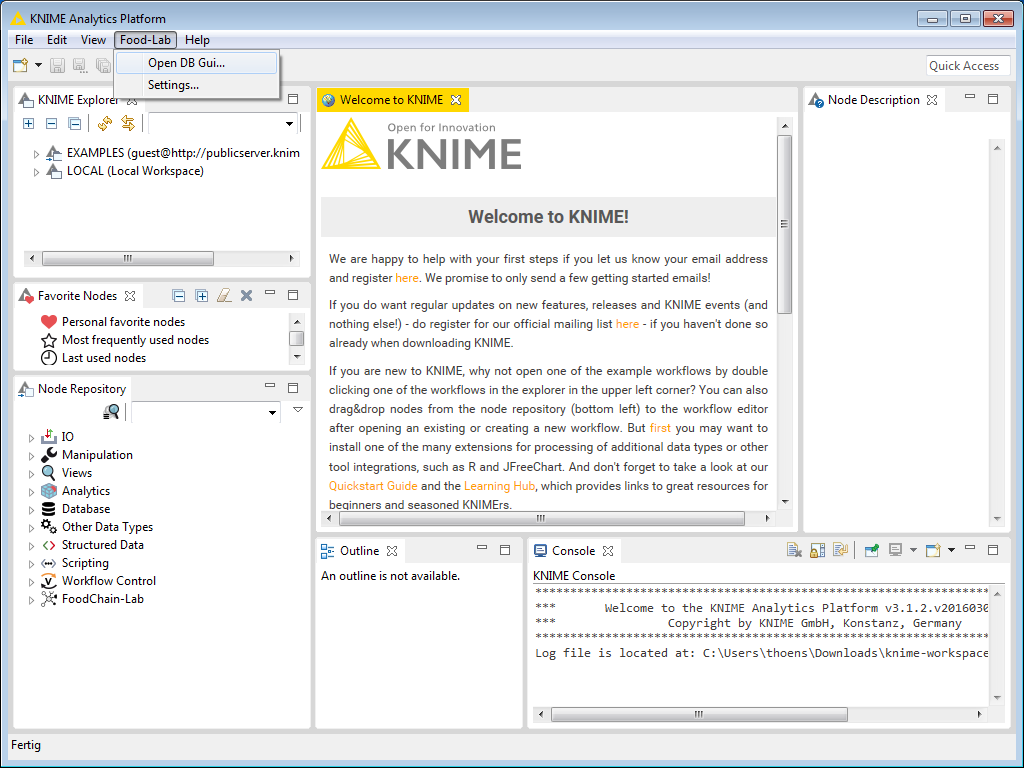
\includegraphics[height=0.6\textheight]{1.png}
	\end{center}
	\begin{itemize}
		\item Wählen Sie \textbf{Food-Lab $>$ Open DB Gui...} in der Menüleiste um das Datenbank-Fenster zu öffnen.
	\end{itemize}
\end{frame}

\subsection{2}
\begin{frame}
	\begin{center}
  		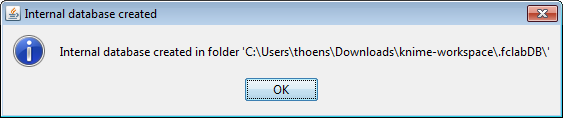
\includegraphics[width=0.9\textwidth]{2.png}
	\end{center}
	\begin{itemize}
		\item Falls Sie eine Meldung bekommen, dass eine interne Datenbank erstellt wurde, klicken Sie \textbf{OK}.
	\end{itemize}
\end{frame}

\subsection{3}
\begin{frame}
	\begin{center}
  		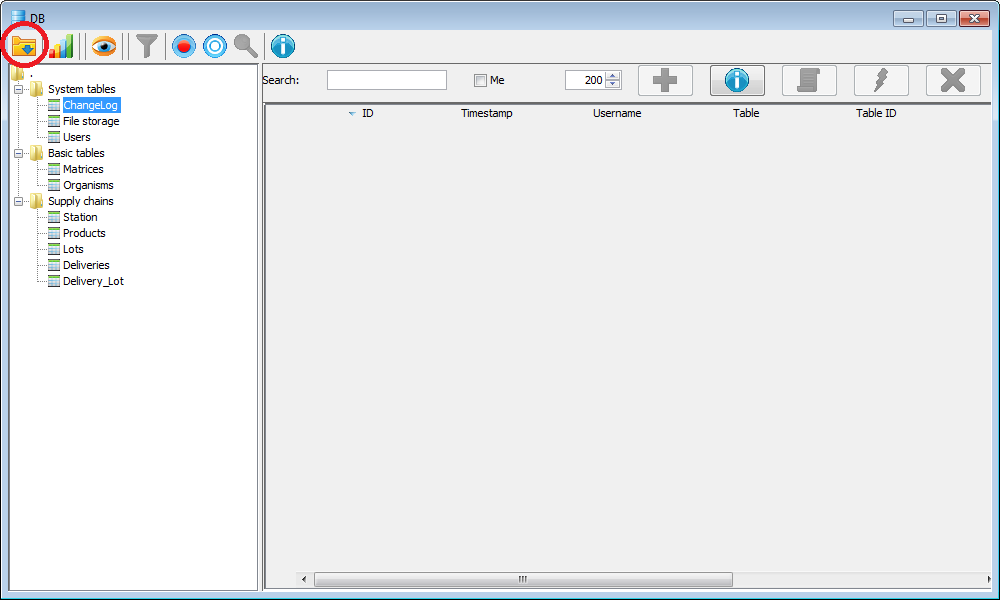
\includegraphics[height=0.6\textheight]{3.png}
	\end{center}
	\begin{itemize}
		\item Im Datenbank-Fenster klicken Sie den \textbf{Table import}-Button links oben.
	\end{itemize}
\end{frame}

\subsection{4}
\begin{frame}
	\begin{center}
  		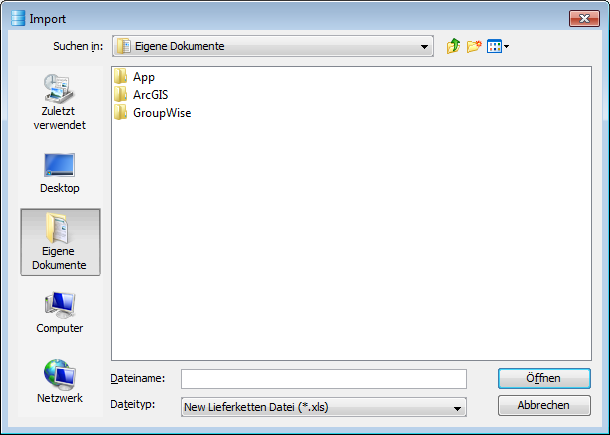
\includegraphics[height=0.6\textheight]{4.png}
	\end{center}
	\begin{itemize}
		\item Es öffnet sich nun ein Dateidialog, in dem *.xls Dateien im FoodChain-Lab Format ausgewählt werden können.
	\end{itemize}
\end{frame}

\subsection{5}
\begin{frame}
	\begin{center}
  		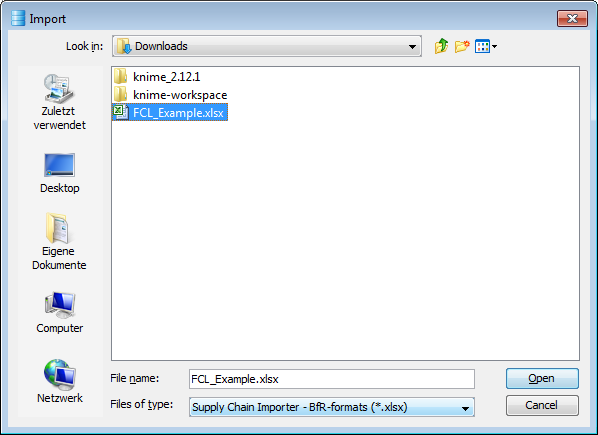
\includegraphics[height=0.6\textheight]{5.png}
	\end{center}
	\begin{itemize}
		\item Laden Sie die Beispieldatei von \url{https://github.com/SiLeBAT/BfROpenLabResources/raw/master/GitHubPages/documents/fake_data.xls}.
		\item Wählen Sie diese Datei im Dialog aus und drücken Sie \textbf{Open}.
	\end{itemize}
\end{frame}

\subsection{6}
\begin{frame}
	\begin{center}
  		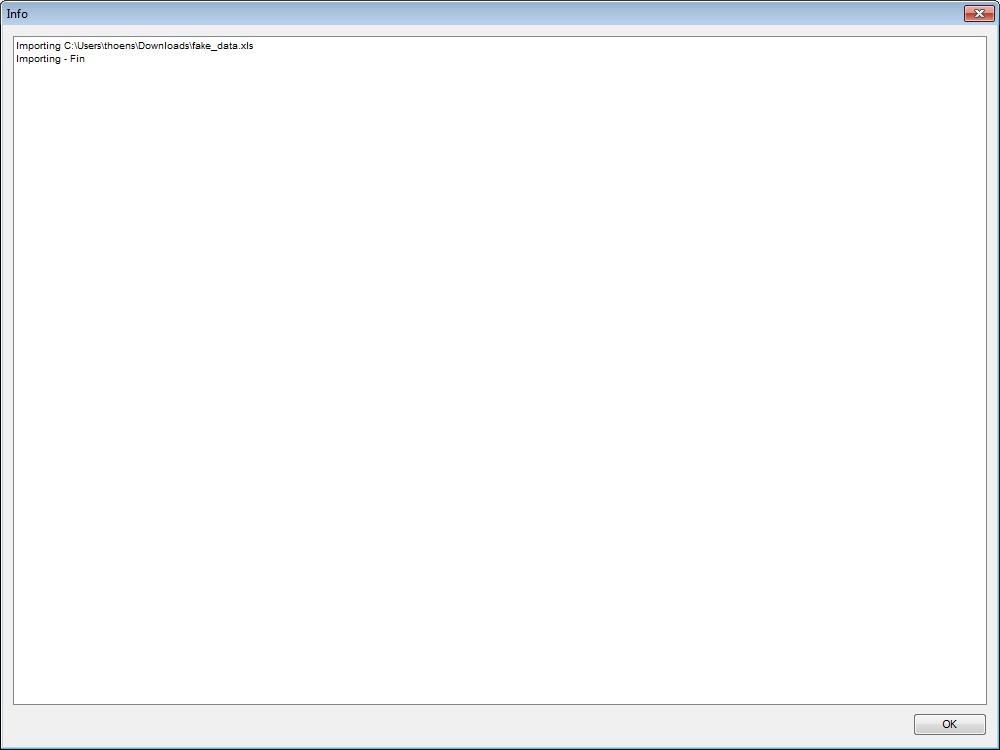
\includegraphics[height=0.6\textheight]{6.png}
	\end{center}
	\begin{itemize}
		\item When der Import beendet ist, werden Sie einen Dialog mit Fehlern/Warnungen sehen, die beim Importieren aufgetreten sind.
		\item Es sind keine Fehler aufgetreten, also drücken Sie einfach \textbf{OK}.
	\end{itemize}
\end{frame}

\subsection{7}
\begin{frame}
	\begin{center}
  		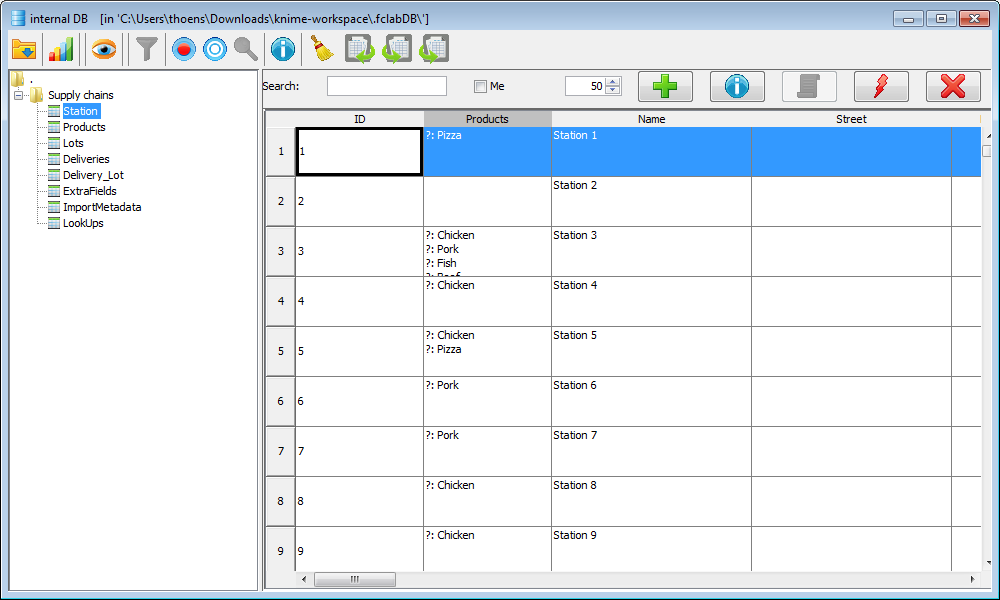
\includegraphics[height=0.6\textheight]{7.png}
	\end{center}
	\begin{itemize}
		\item Im Datenbank-Fenster können Sie sich die importierten Daten nun anschauen, nach Duplikaten suchen usw..
		\item Schließen Sie den Dialog.
	\end{itemize}
\end{frame}

\subsection{8}
\begin{frame}
	\begin{center}
  		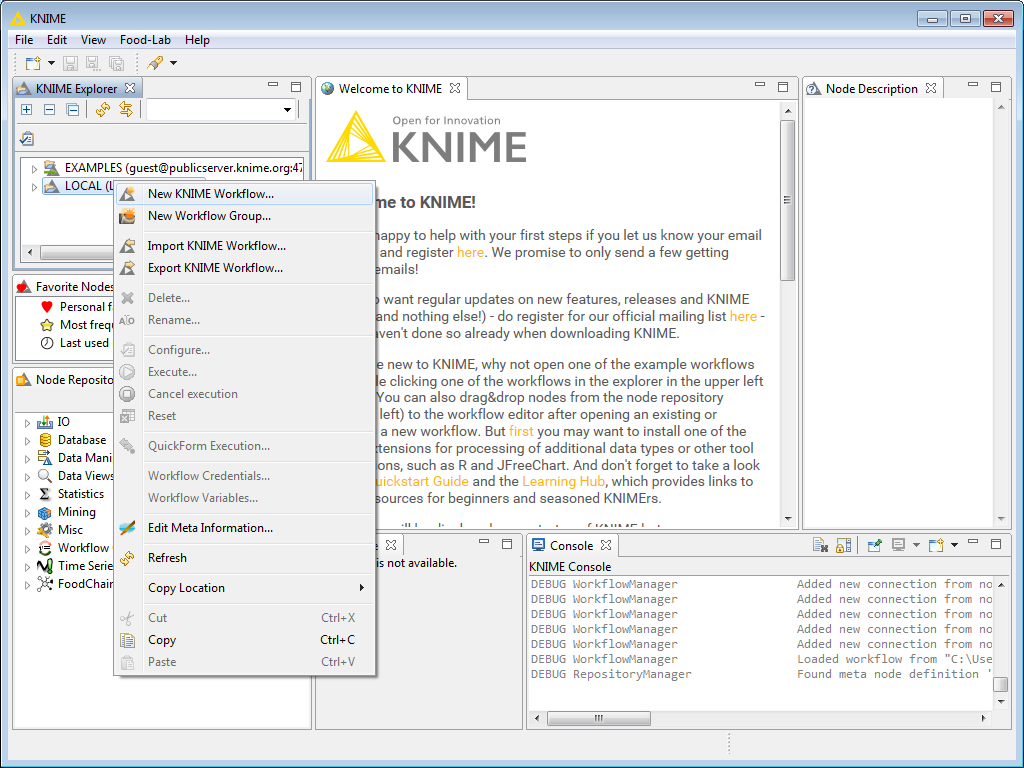
\includegraphics[height=0.6\textheight]{8.png}
	\end{center}
	\begin{itemize}
		\item Nun werden wir einen Workflow erzeugen, der die importierten Daten nutzt.
		\item Machen Sie einen Rechtsklick auf \textbf{LOCAL} im \textbf{KNIME Explorer} and wählen Sie \textbf{New KNIME Workflow...}
	\end{itemize}
\end{frame}

\subsection{9}
\begin{frame}
	\begin{center}
  		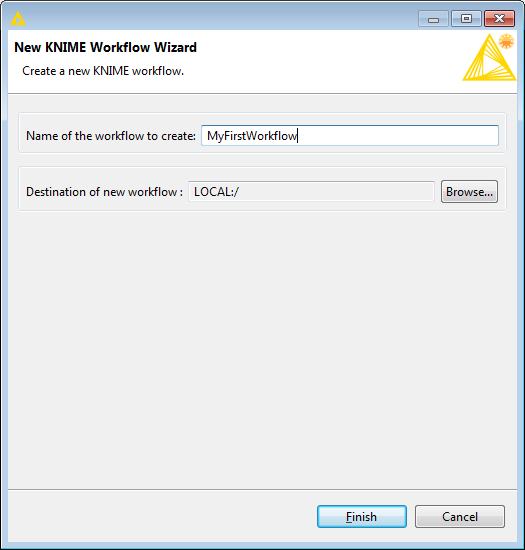
\includegraphics[height=0.6\textheight]{9.png}
	\end{center}
	\begin{itemize}
		\item Im erscheinenden Dialog wählen Sie als Name "My First Workflow" and klicken Sie \textbf{Finish}.		
	\end{itemize}
\end{frame}

\subsection{10}
\begin{frame}
	\begin{center}
  		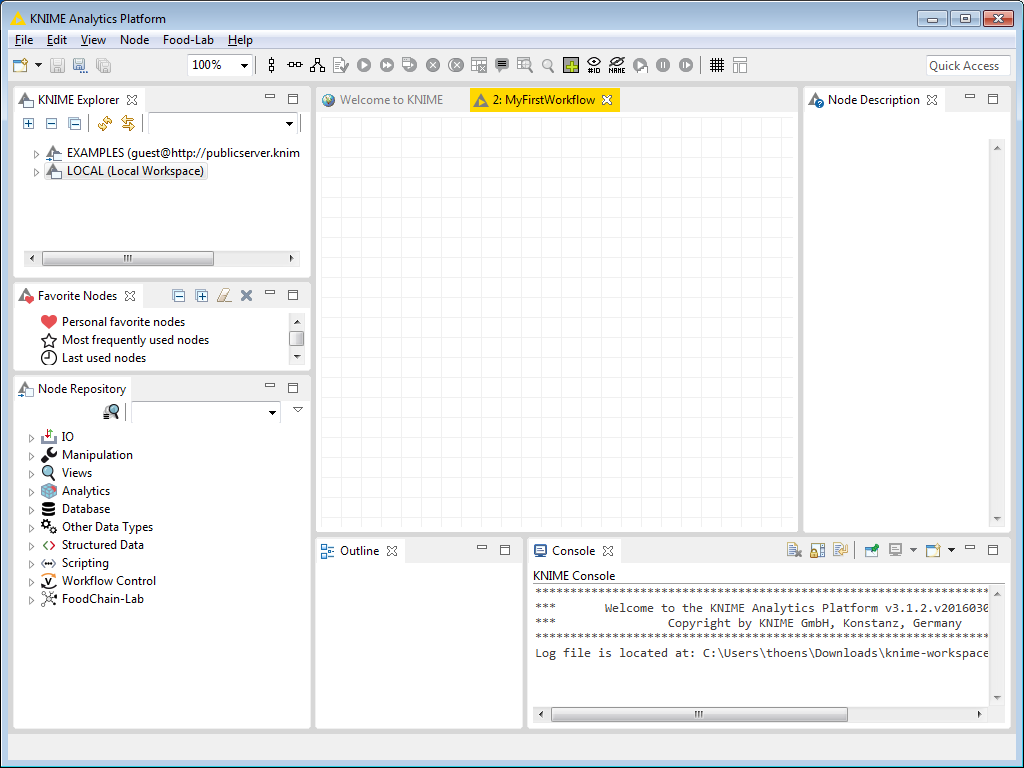
\includegraphics[height=0.6\textheight]{10.png}
	\end{center}
	\begin{itemize}
		\item Der erzeugte Workflow wird im Editor in der Mitte des Fensters erscheinen.
	\end{itemize}
\end{frame}

\subsection{11}
\begin{frame}
	\begin{center}
  		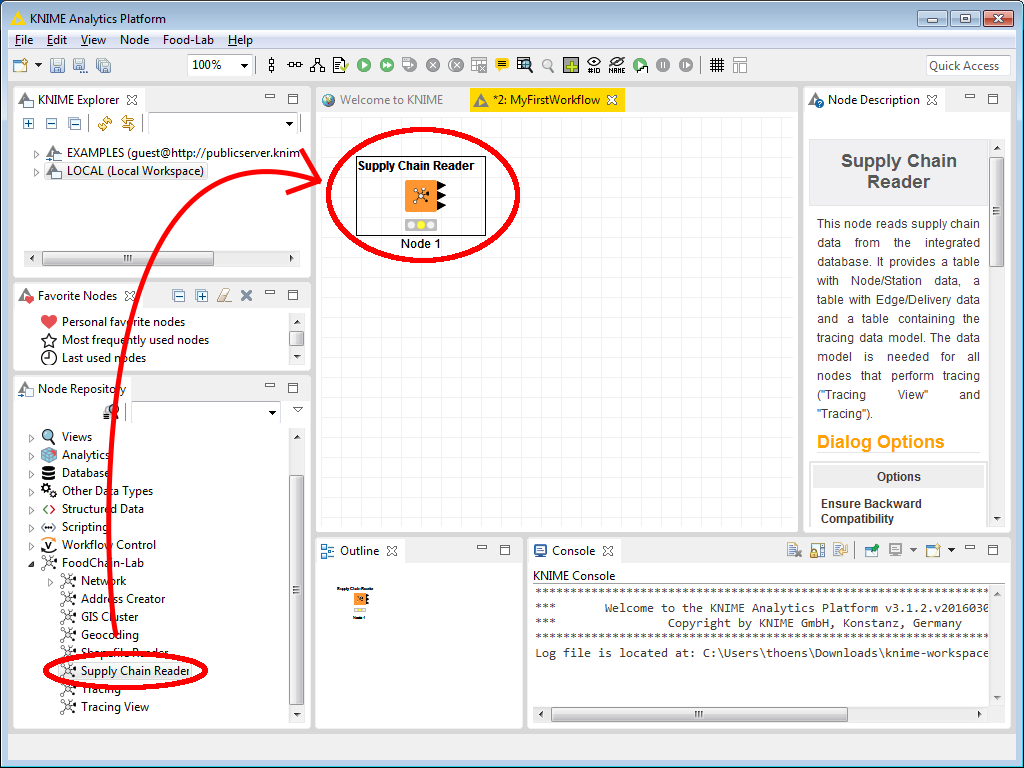
\includegraphics[height=0.6\textheight]{11.png}
	\end{center}
	\begin{itemize}
		\item Ziehen Sie den \textbf{Supply Chain Reader} aus dem \textbf{Node Repository} in den Workflow.
	\end{itemize}
\end{frame}

\subsection{12}
\begin{frame}
	\begin{center}
  		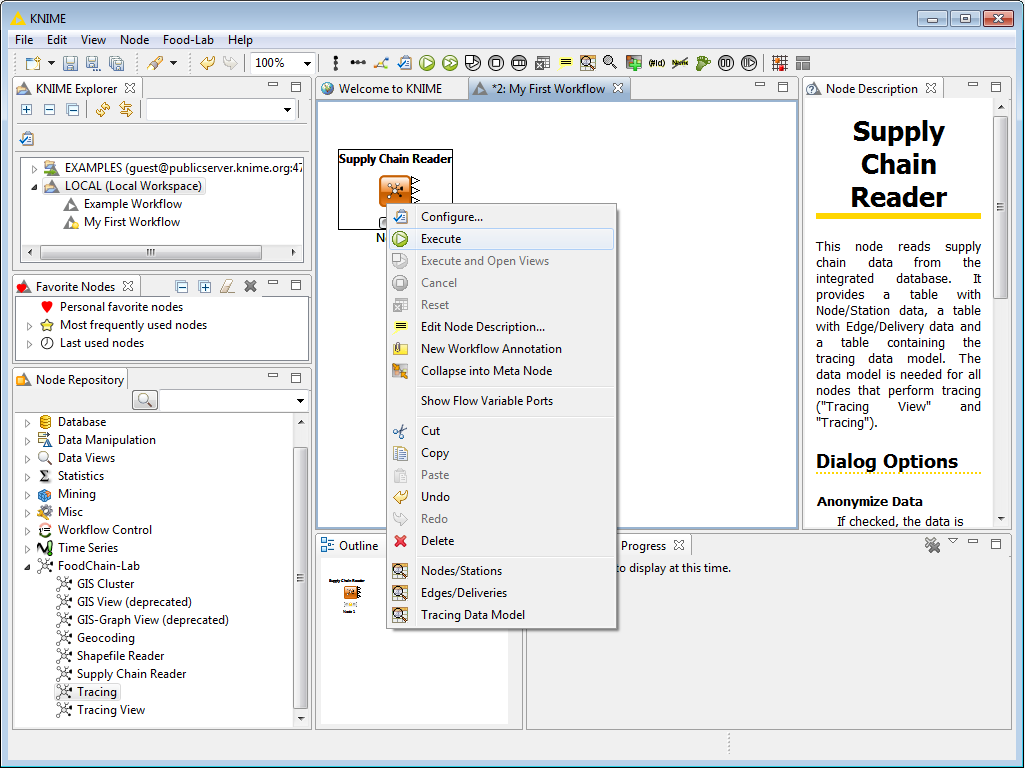
\includegraphics[height=0.6\textheight]{12.png}
	\end{center}
	\begin{itemize}
		\item Der \textbf{Supply Chain Reader} muss nicht konfiguriert werden.
		\item Also machen Sie einen Rechtsklick auf den Knoten und wählen Sie \textbf{Execute} um den Knoten auszuführen.
	\end{itemize}
\end{frame}

\subsection{13}
\begin{frame}
	\begin{center}
  		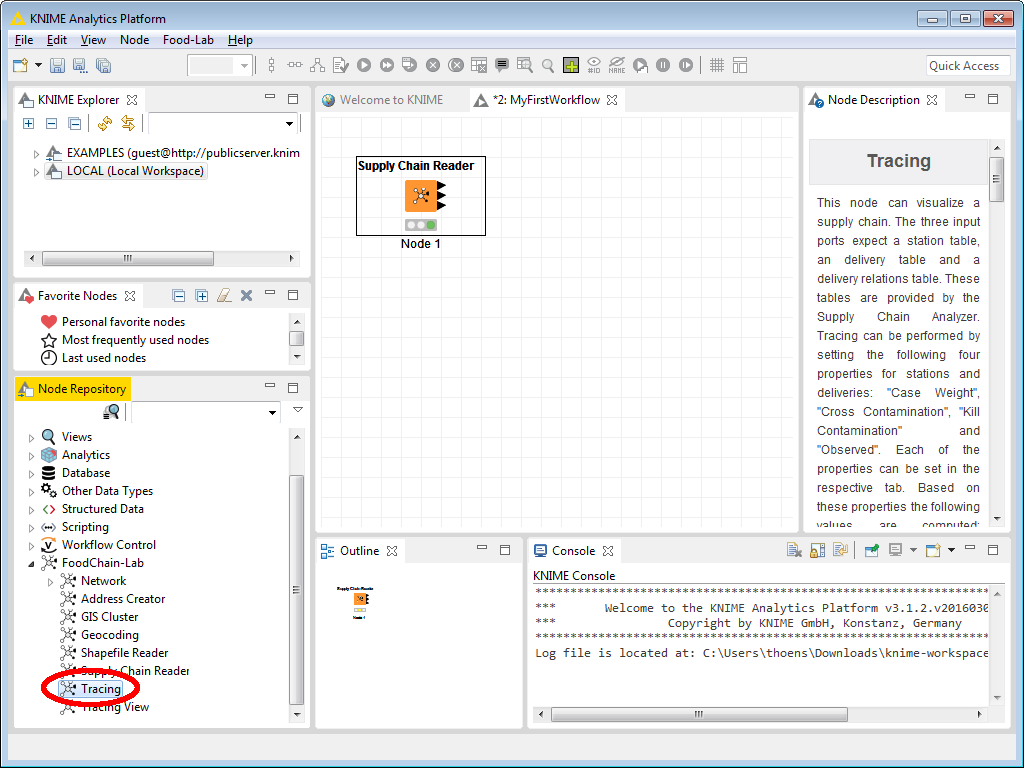
\includegraphics[height=0.6\textheight]{13.png}
	\end{center}
	\begin{itemize}
		\item Der \textbf{Supply Chain Reader} hat nun alle Daten aus der internen Datenbank gelesen.
		\item Selektieren Sie den \textbf{Supply Chain Reader} im Workflow (sodass ein Rechteck um den Knoten erscheint) machen Sie einen Doppelklick auf den \textbf{Tracing}-Knoten im \textbf{Node Repository}.
	\end{itemize}
\end{frame}

\subsection{14}
\begin{frame}
	\begin{center}
  		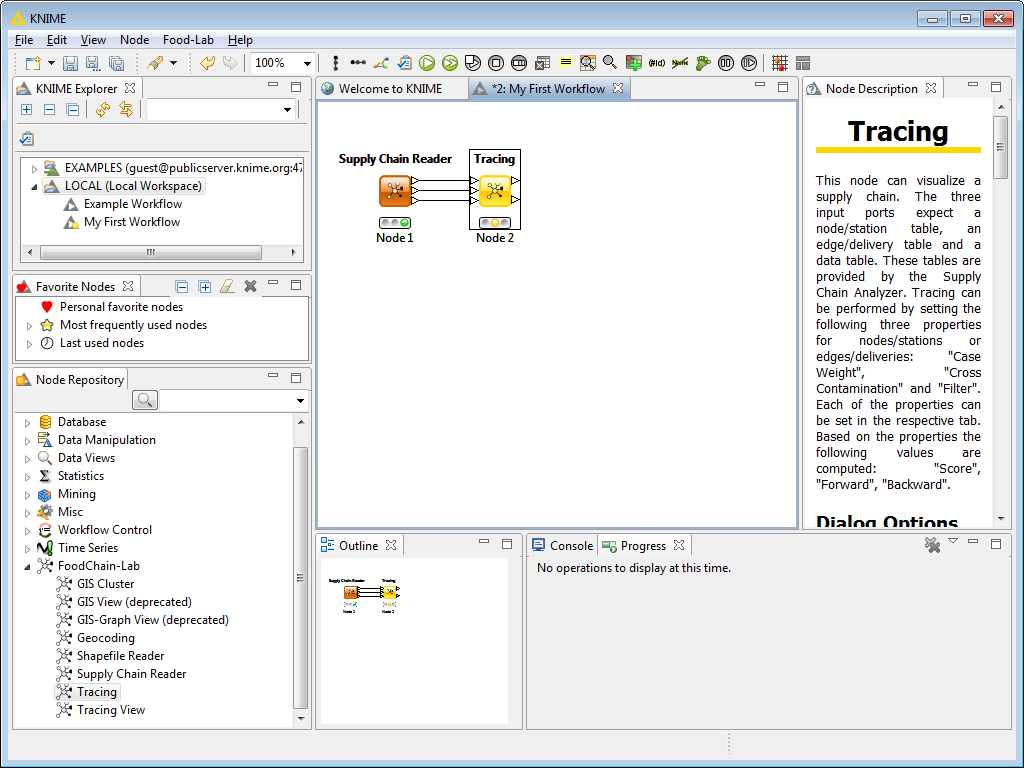
\includegraphics[height=0.6\textheight]{14.png}
	\end{center}
	\begin{itemize}
		\item Der \textbf{Tracing}-Knoten sollte nun im Workflow erscheinen and alle Eingabe-Ports sollten automatisch mit dem \textbf{Supply Chain Reader} verbunden werden.
		\item Machen Sie einen Doppelklick auf den \textbf{Tracing}-Knoten um diesen zu konfigurieren.
	\end{itemize}
\end{frame}

\subsection{15}
\begin{frame}
	\begin{center}
  		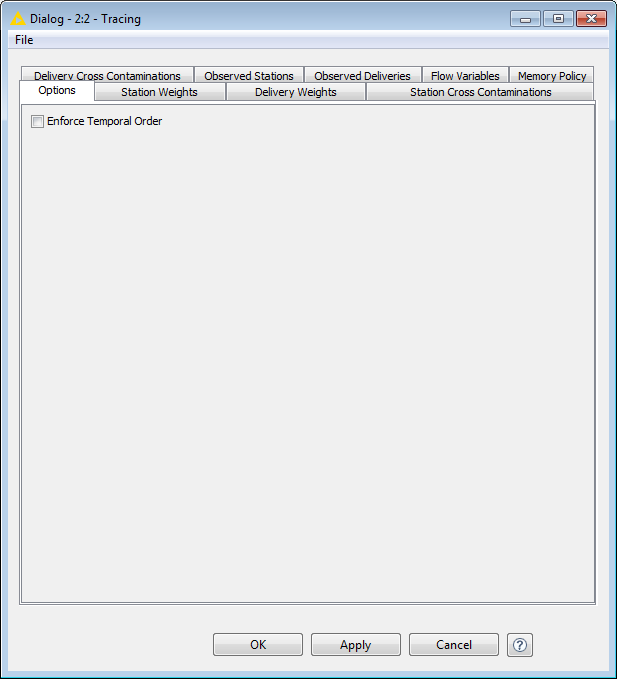
\includegraphics[height=0.5\textheight]{15.png}
	\end{center}
	\begin{itemize}
		\item Im oberen Bereich des Dialogs sehen Sie die Tabs für die einzelnen Parameter.
		\item "Weight" und "Cross Contamination" können für Stationen/Lieferungen gesetzt werden. Basierend darauf wird für jede Station/Lieferung ein "Score" berechnet.
		\item Zusätzlich können Stationen/Lieferungen mit dem Attribut "Observed" versehen werden.
		\item Wählen Sie den \textbf{Station Weights}-Tab.
	\end{itemize}
\end{frame}

\subsection{16}
\begin{frame}
	\begin{center}
  		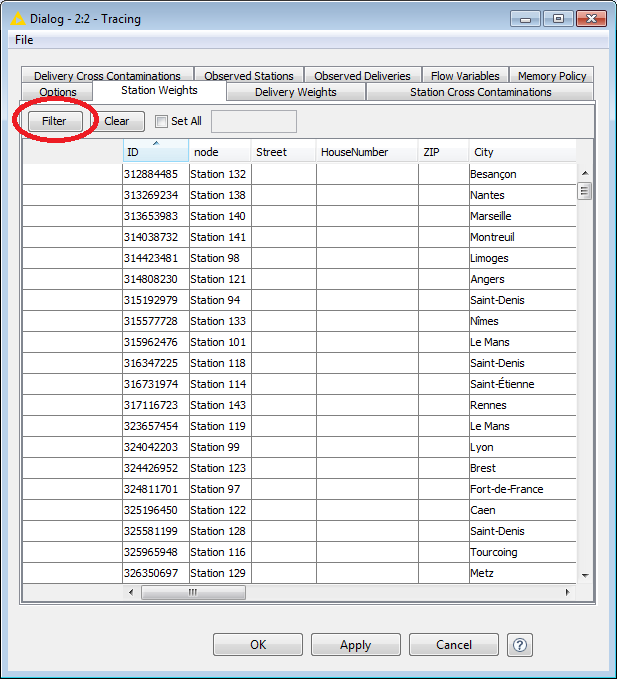
\includegraphics[height=0.5\textheight]{16.png}
	\end{center}
	\begin{itemize}
		\item Eine Tabelle mit allen verfügbaren Stationen erscheint.
		\item Das Gewicht ("Weight") kann in der ganz linken Spalte vergeben werden.
		\item Da es sehr ineffizient ist durch eine so große Anzahl von Station zu scrollen, können wir einen Filter setzen um nur die gewünschten Station anzeigen zu lassen.
		\item Klicken Sie auf \textbf{Filter}.
	\end{itemize}
\end{frame}

\subsection{17}
\begin{frame}
	\begin{center}
  		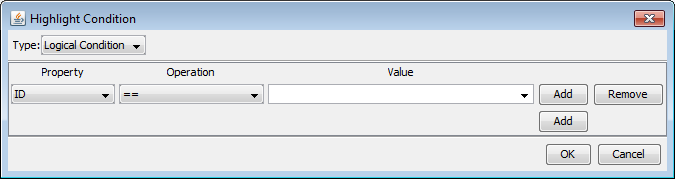
\includegraphics[width=0.9\textwidth]{17.png}
	\end{center}
	\begin{itemize}
		\item In diesem Dialog können Sie festlegen, welche Stationen in der Tabelle erscheinen sollen.
	\end{itemize}
\end{frame}

\subsection{18}
\begin{frame}
	\begin{center}
  		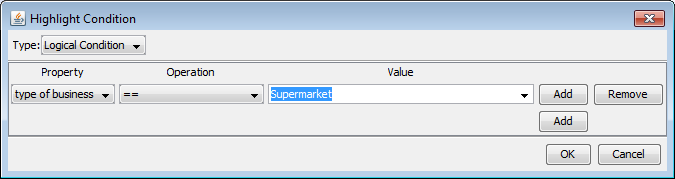
\includegraphics[width=0.9\textwidth]{18.png}
	\end{center}
	\begin{itemize}
		\item Wir wollen nur für Supermärkte Gewichte vergeben, da dort kontaminierte Produkte gefunden wurden.
		\item Wählen Sie "type of business" bei \textbf{Property} und "Supermarket" bei \textbf{Value}.
		\item Klicken Sie \textbf{OK}.
	\end{itemize}
\end{frame}

\subsection{19}
\begin{frame}
	\begin{center}
  		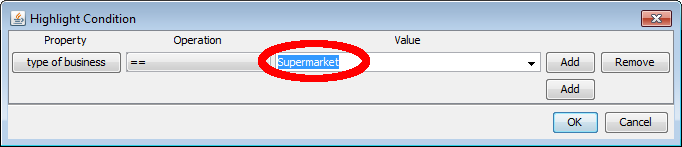
\includegraphics[height=0.6\textheight]{19.png}
	\end{center}
	\begin{itemize}
		\item Nun sehen Sie nur Supermärkte in der Tabelle.
	\end{itemize}
\end{frame}

\subsection{20}
\begin{frame}
	\begin{center}
  		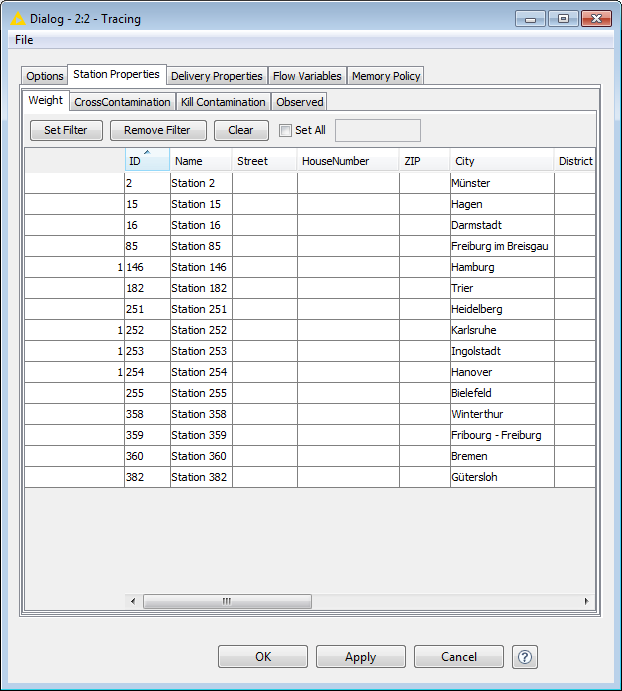
\includegraphics[height=0.6\textheight]{20.png}
	\end{center}
	\begin{itemize}
		\item Vergeben Sie ein Gewicht von "1" an die Supermärkte in "Hamburg", "Ingolstadt" und "Münster", da dort kontaminierte Produkte gefunden wurden.
		\item Klicken Sie auf \textbf{OK} um die Eingabe zu beenden.
	\end{itemize}
\end{frame}

\subsection{21}
\begin{frame}
	\begin{center}
  		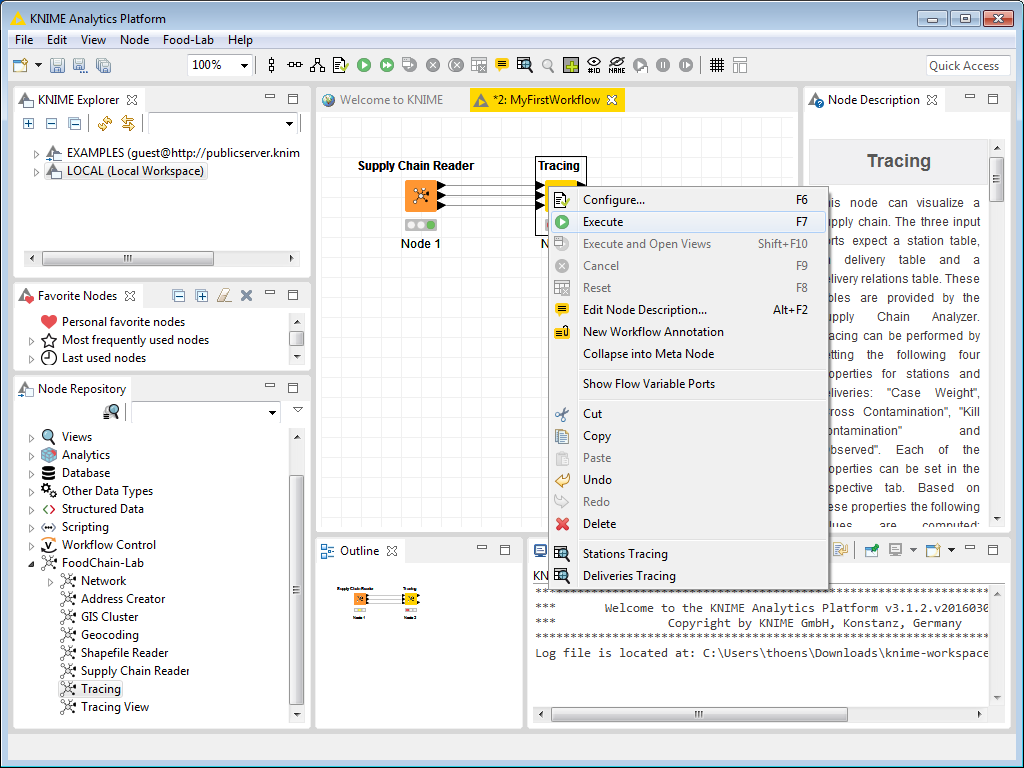
\includegraphics[height=0.6\textheight]{21.png}
	\end{center}
	\begin{itemize}
		\item Machen Sie einen Rechtsklick auf den \textbf{Tracing}-Knoten und wählen Sie \textbf{Execute} um den Knoten auszuführen.
	\end{itemize}
\end{frame}

\subsection{22}
\begin{frame}
	\begin{center}
  		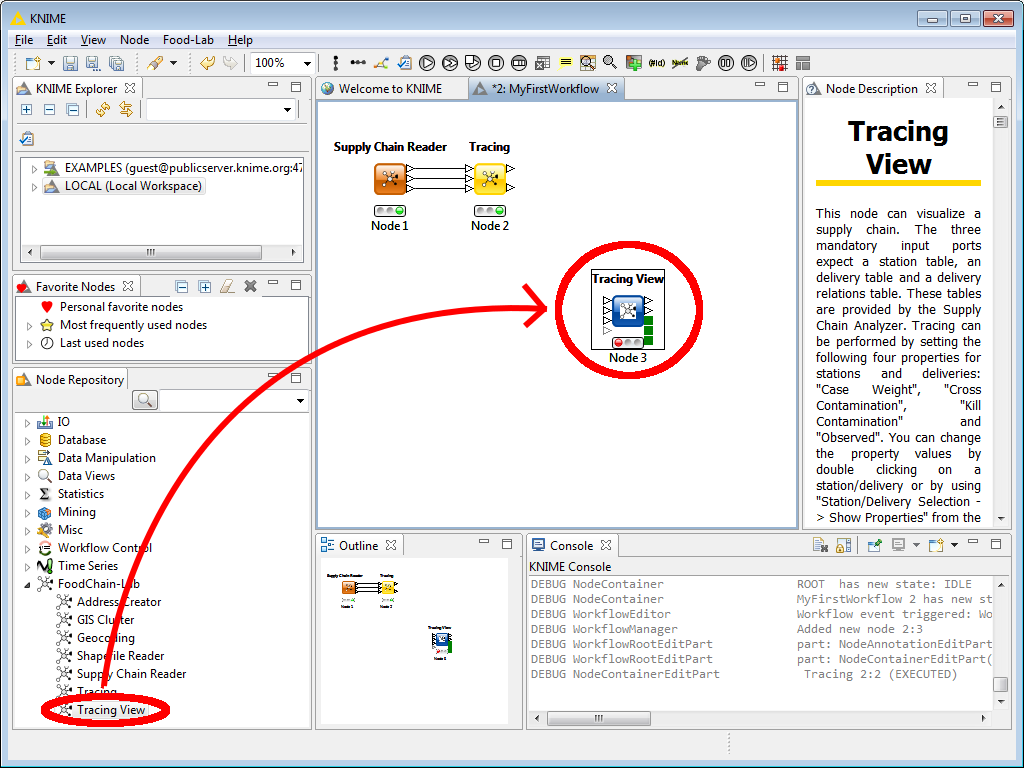
\includegraphics[height=0.6\textheight]{22.png}
	\end{center}
	\begin{itemize}
		\item Ziehen Sie den \textbf{Tracing View} aus dem \textbf{Node Repository} in den Workflow.
	\end{itemize}
\end{frame}

\subsection{23}
\begin{frame}
	\begin{center}
  		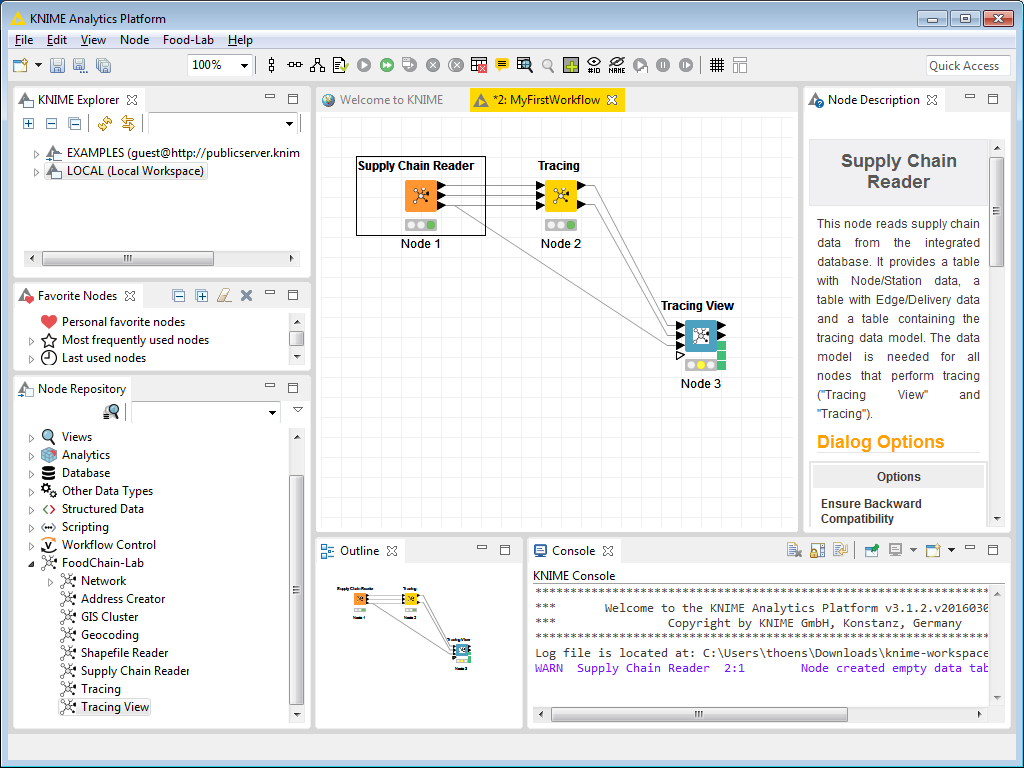
\includegraphics[height=0.5\textheight]{23.png}
	\end{center}
	\begin{itemize}
		\item Verbinden Sie die Ausgabe-Ports des \textbf{Tracing}-Knotens mit den beiden ersten Eingabe-Ports vom \textbf{Tracing View}.
		\item Verbinden Sie den dritten Ausgabe-Port vom \textbf{Supply Chain Reader} mit dem dritten Eingabe-Port vom \textbf{Tracing View}.
		\item Nun öffnen Sie den \textbf{Tracing View} and analysieren Sie die Daten. Dies wird im zweiten Teil des Tutorials gezeigt.
	\end{itemize}
\end{frame}

\end{document}